\documentclass{beamer}
%\documentclass[aspectratio=169]{beamer}
%
\mode<presentation>
{
  \usetheme{default}      
  \usecolortheme{default}
  \usefonttheme{default} 
  \setbeamertemplate{navigation symbols}{}
  \setbeamertemplate{caption}[numbered]
} 

\usepackage[english]{babel}
\usepackage[utf8x]{inputenc}

\title[Classification]{Introduction to Machine Learning}
\subtitle{Lecture 2: Classification}
\author{Alexis Zubiolo\newline\texttt{alexis.zubiolo@gmail.com}}
\institute{Data Science Team Lead @ Adcash}
\date{October 20, 2016}

\begin{document}

\begin{frame}
  \titlepage
\end{frame}

\begin{frame}{Classification in Machine Learning}
This lecture is about classification in Machine learning.
\vfill
\textbf{Reminder}: In classification, the output $y$ is \textbf{categorical}.
\vfill
\textbf{Examples}:
\begin{itemize}
	\item Mail classification: $y =$ spam or $y =$ not spam
	\item Object recognition: $y =$ apple, $y =$ car, \ldots
\end{itemize}
\end{frame}

\begin{frame}{Classification in Machine Learning: Applications}
Domains of application:
\begin{itemize}
	\item Medicine
	\item Image/video classification
	\item Face recognition/identification
	\item Spam filtering
	\item Fraud detection
	\item Click prediction
	\item Product recommendation
	\item Robotics
	\item Language processing
	\item Web search
	\item \ldots and many others
\end{itemize}
\end{frame}
%
\begin{frame}{Support Vector Machines, Decision Trees}
In this course, we will see
\begin{itemize}
	\item Support Vector Machines (SVMs)
	\item Decision Trees (DTs) / Boosting
\end{itemize}
\vfill
Why? Because the concepts behind these classifiers are quite intuitive.
\end{frame}
%
\begin{frame}
\begin{center}
\Huge{Support Vector Machines}
\end{center}
\end{frame}
%
\begin{frame}{Support Vector Machines: History and intuition}
A few historical facts about SVMs:
\begin{itemize}
	\item First introduced by \textbf{Cortes and Vapnik} in 1995 from AT\&T Bell labs (paper called Support-Vector Networks)
	\item Quickly became state of the art in many areas
	\item Received a lot of attention since then
	\item Still a widely used classifier
\end{itemize}
\vfill 
Intuitive idea behind SVMs: Find the linear separator with the widest margin.
\end{frame}
%
\begin{frame}{SVM: Widest margin}
\begin{figure}
\centering
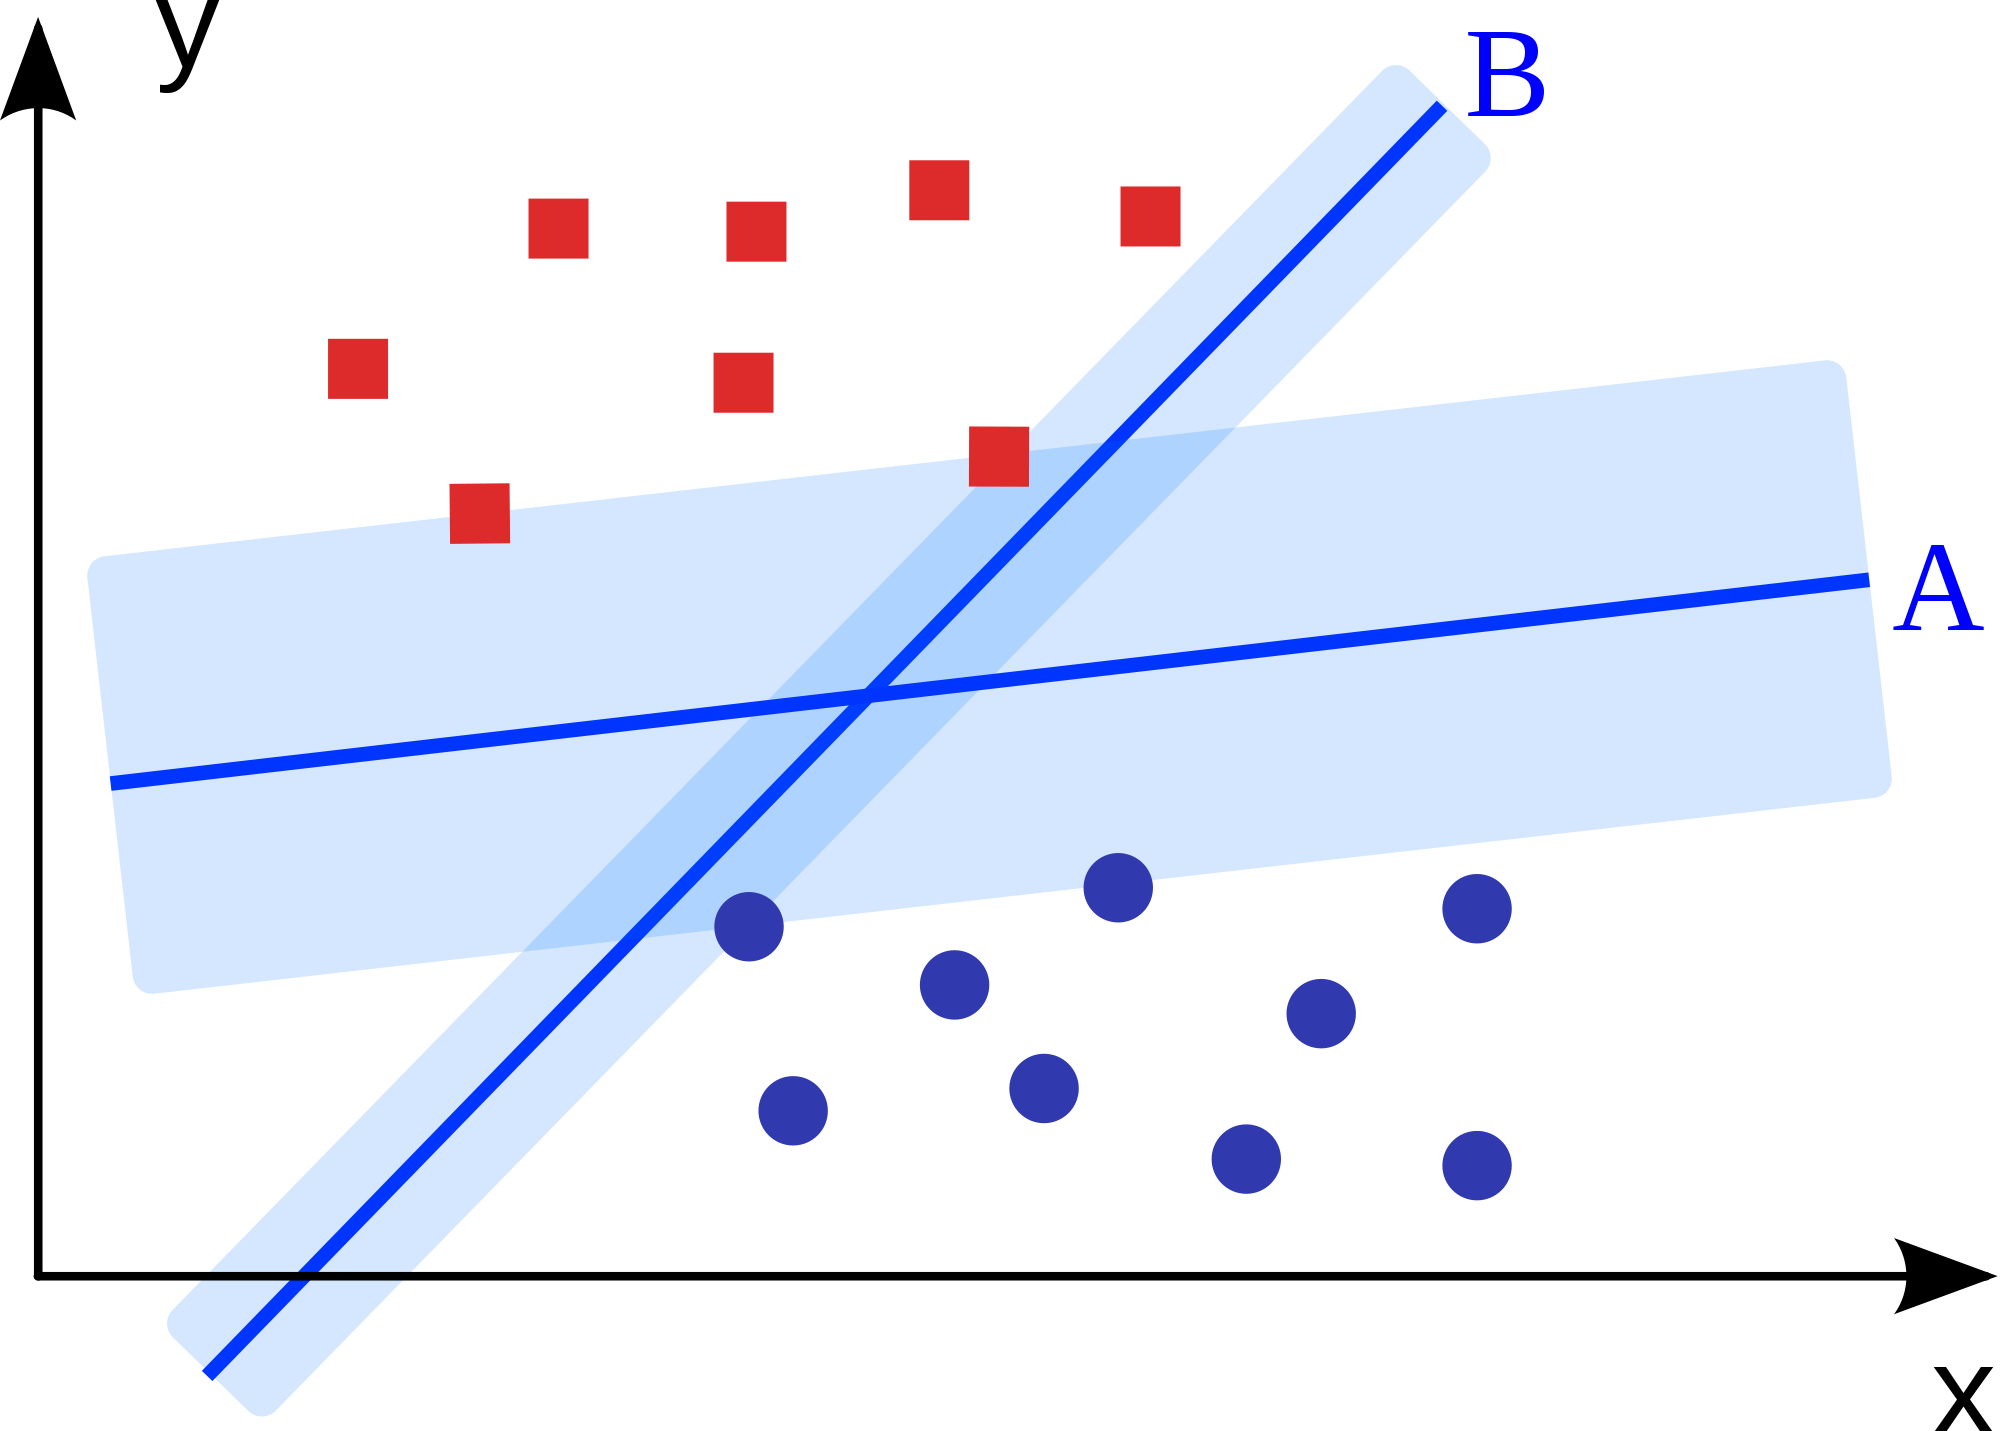
\includegraphics[width=\textwidth]{images/svm_margin.png}
\end{figure}
\end{frame}
%
\begin{frame}{SVM: Widest margin}
Among all the possible separators, SVM chooses the one \textbf{with the widest margin}.
\vfill
\pause
Why? Intuitively, a wide margin leads to a good \textbf{generalization of the classifier} on new points.
\end{frame}
%
\begin{frame}{SVM: The kernel trick}
\vfill
So far, the SVM we have seen is a \textit{linear classifier}: It aims at finding a linear separation between the 2 classes. What if they are \textbf{not linearly separable}? 
\vfill
Example: See example on the board
\vfill
What to do in this case? \pause The \textbf{kernel trick} is an option.
\vfill
\end{frame}
%
\begin{frame}{SVM: The kernel trick}
The kernel trick consists in \textbf{mapping the features $x$ to a space of higher dimensionality} where the data is (hopefully) linearly separable.
\pause
\begin{figure}
\centering
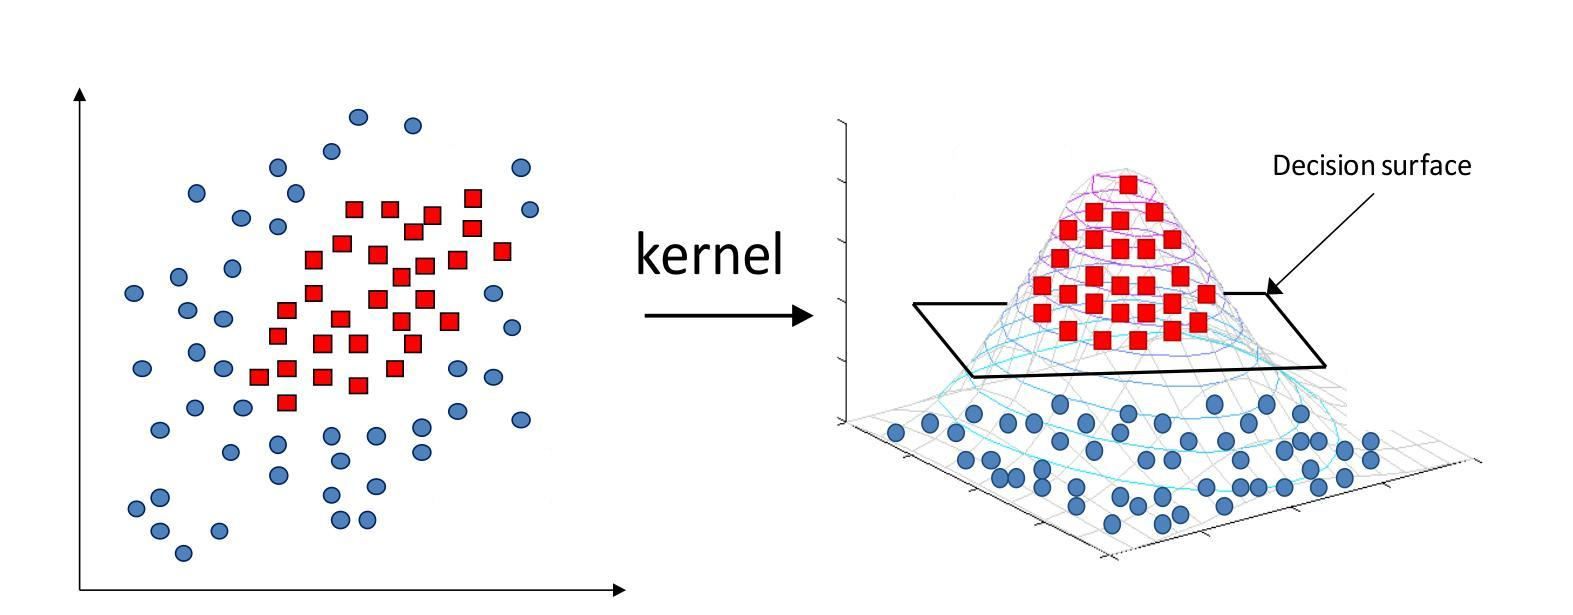
\includegraphics[width=\textwidth]{images/kernel_trick_3d.jpg}
\end{figure}

Most commonly used kernels: \textbf{Gaussian} (aka RBF) and \textbf{polynomial} kernels.
\pause
\vfill \textbf{Note}: Adding a kernel leads to \textbf{extra parameters}.
\end{frame}
%
\begin{frame}{SVM: Soft margin}
Not tolerating points within the margin may lead to really \textbf{``thin'' separators}, and then to \textbf{bad generalization}.
\pause
\vfill 
It is possible to tolerate some violation of the margin. The idea is to find a \textbf{proper trade-off} between width of the margin and violation tolerance.
\pause
\vfill 
Ideally, we want 
\begin{itemize}
	\item a wide margin
	\item little to no violation of the margin
\end{itemize}
\pause
\vfill 
but in practice, it is almost not possible, for example because:
\begin{itemize}
	\item The data may not be linearly separable (even after the kernel trick)
	\item There is noise in the data
\end{itemize}
\end{frame}
%
\begin{frame}{SVM: Soft margin}
\begin{figure}
\centering
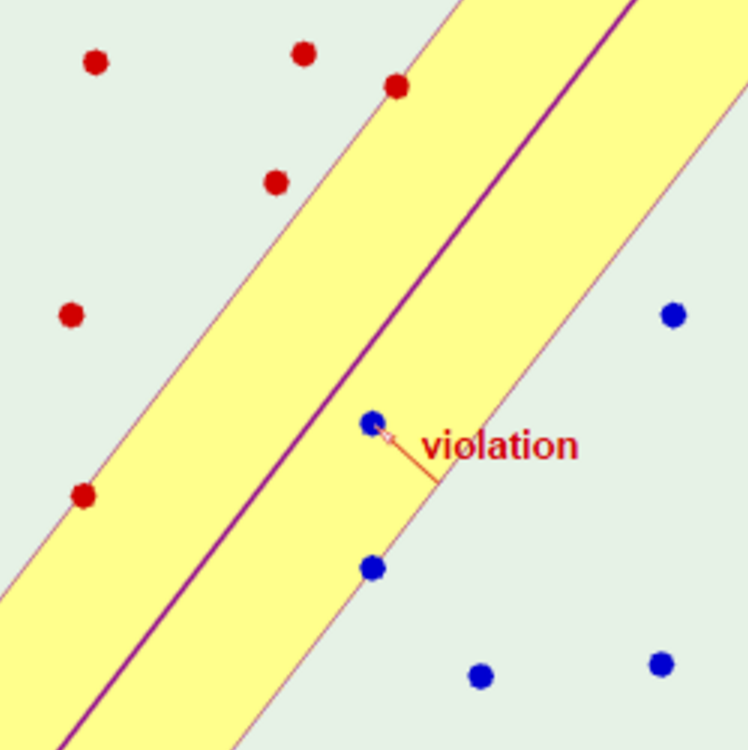
\includegraphics[width=0.75\textwidth]{images/soft_margin.png}
\end{figure}
\end{frame}

\begin{frame}{SVM: Recap}
SVM consists in:
\begin{itemize}
	\item Finding the widest separator
	\item Using kernels if the data is not linearly separable
	\item Using soft margin 
\end{itemize}
\vfill
It has parameters that need to be tuned:
\begin{itemize}
	\item Soft margin trade-off: $C$
	\item Kernel parameter:
	\begin{itemize}
		\item Degree $d$ for polynomial kernels
		\item The standard deviation $\sigma$ for RBF kernels
	\end{itemize}
\end{itemize}

\end{frame}
%
\begin{frame}{SVM}
\vfill
\Large{Interactive demonstration (c) Andrej Karpathy}
\vfill
\end{frame}
%
\begin{frame}{SVM for multiclass classification}
\vfill
What we have seen so far works for \textit{binary classification} (2 classes). What if we have \textbf{3 classes or more}?
\vfill
\pause 
Several possible extensions. Some of the most popular ones:
\begin{itemize}
	\item One against one classification
	\item One against all classification
\end{itemize}
\vfill
\textbf{Note}: These strategies apply to any binary classifier.
\vfill
\end{frame}
%
\begin{frame}{One against one classification}
\textbf{Idea}: 
\begin{itemize}
	\item Compute a classifier \textbf{for all pairs} of classes.
	\item \textbf{Apply all these classifiers} to the new point. Store the predicted classes.
	\item \textbf{Majority vote}: Return the class with the highest number of votes
\end{itemize}

\end{frame}
%
\begin{frame}{One against all classification}
\vfill
\textbf{Note}: It is also called \textit{one against rest classification}.
\vfill
\textbf{Idea}: For each class, split the set of classes into two meta classes
\begin{itemize}
	\item The considered class
	\item The union of all the other classes
\end{itemize}
and compute a classifier for all these possibilities.
Apply all these classifiers to a (new) given point.
\vfill
Final decision: More complicated than for one-versus-one
\end{frame}
%
\begin{frame}
\begin{center}
\Huge{Decision Trees}
\end{center}
\end{frame}

\begin{frame}{Decision Trees / Boosting}
\vfill
\textbf{Note}: DTs and Boosting are different algorithms, but they share some common ideas.
\vfill
\textbf{Idea}: \textbf{Combining weak classifiers} to get a more robust classifier.
\vfill
\textbf{How}? By applying these \textit{weak} classifier successively. 
\end{frame}

\begin{frame}{DTs/Boosting: Toy example}
\begin{figure}
\centering
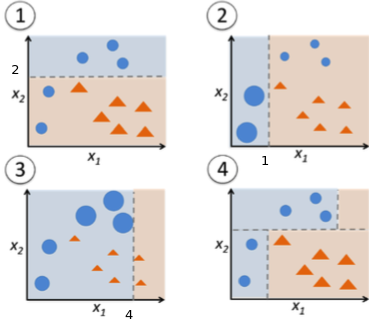
\includegraphics[width=0.75\textwidth]{images/boosting.png}
\end{figure}
(step 4 is optional). Try to guess the resulting tree.
\end{frame}

\begin{frame}{DTs: visualization with sklearn}
\begin{figure}
\centering
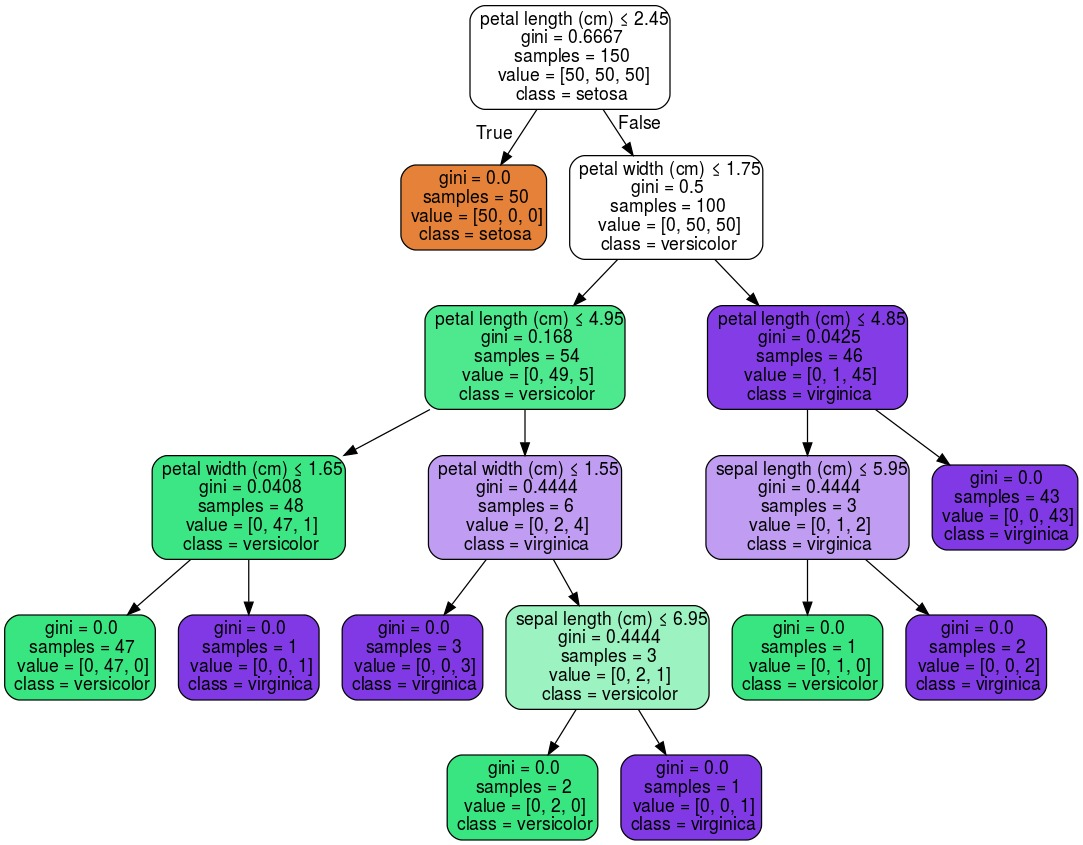
\includegraphics[width=0.75\textwidth]{images/iris_tree.jpg}
\end{figure}
\end{frame}

\begin{frame}{Decision Trees}
\vfill
\Large{Interactive demonstration (c) Andrej Karpathy}
\vfill
\end{frame}

\begin{frame}{DTs/boosting recap}

\textbf{Goal}: Build a tree of simple classifier to obtain a more sophisticated classifier.

There are \textbf{several parameters} that have to be set:
\begin{itemize}
	\item The \textbf{number of trees}
	\item The \textbf{maximum depth} of the trees
	\item The \textbf{number of decision} per node
\end{itemize}

\end{frame}

\begin{frame}{Conclusion}
We've seen two popular classifiers:
\begin{itemize}
	\item Support Vector Machines
	\item Decision Trees
\end{itemize}

A few remarks before we finish:
\begin{itemize}
	\item These classifiers (and others as well) rely on a few parameters that have \textbf{a huge impact} on the quality of the resulting classifier. Example: soft-margin parameter for SVMs, number of trees for DTs. 
	\item Parameters others than accuracy have to be taken into account when choosing the parameters. Example: More tree may lead to a better classifier but it involves more computation also. A proper trade-off has to be found depending on the application.
\end{itemize}
\end{frame}

\begin{frame}
\begin{center}
\Huge{Thank you! Questions?}
\end{center}
\end{frame}

\end{document}